\documentclass[a4paper,12pt]{article}
 \usepackage[utf8]{inputenc}
 \usepackage[french]{babel}
 \usepackage[T1]{fontenc}
 %IMAGE
 \usepackage{graphicx}
 \usepackage[export]{adjustbox}

%HEADER AND FOOTER 
\usepackage{fancyhdr}
%\setlength\headheight{26pt} 

\pagestyle{fancy}
\fancyhf{}
\rhead{24/04/2015 - Louis Viot}
\lhead{Synthèse SRLC}
\lfoot{
\includegraphics[scale=0.65]{enseeiht.jpg}}
\rfoot{Page \thepage}

\newcommand{\HRule}{\rule{\linewidth}{0.5mm}}

\begin{document}
\begin{titlepage}
\begin{center}

\textsc{\LARGE ENSEEIHT}\\[1.5cm]

\textsc{\Large Master Systèmes Répartis et Logiciel Critique}\\[0.5cm]

% Title
\HRule \\[0.4cm]
{ \huge \bfseries Synthèse \\[0.4cm] }

\HRule \\[1.5cm]
\end{center}

% Author and supervisor
\vspace{3cm}
\begin{minipage}{0.9\textwidth} \large
\begin{flushleft}
\emph{Auteur:}
Louis \textsc{Viot}\\
\emph{Date:}
\today \\
\end{flushleft}
\end{minipage}
\vspace{6cm}
\begin{center}

\includegraphics[scale=1.5]{enseeiht.jpg}
\end{center}

\end{titlepage}






\newpage
\tableofcontents
\section*{Introduction}
Ce rapport a pour but de résumer notre impression sur ce début de projet long. Notamment ce que l'on ressent par rapport, non pas au développement même d'un point de vu logiciel du projet, à la gestion de projet. Nous aborderons dans ce rapport différents points en rapport au cours de gestion de projet et appliqués à ce projet long. On abordera rapidement mon impression par rapport à l'organisation de l'équipe, la plannification, la gestion des risques et la gestion des réunions.\vspace{3cm}
\subsubsection*{Versions}
\noindent
\texttt{version 0.1} : rédaction du corp du rapport \\
\texttt{version 0.2} : intégration des images \\
\texttt{version 0.9} : traduction en \LaTeX \\
\texttt{version 1.0} : relecture et version finale
\newpage
\section{Contexte du stage}
Dans un réacteur nucléaire se trouve le coeur constitué de crayons de combustible (principalement de plutonium et d'uranium). Ces crayons sont assemblés à l'aide de gaines et sont placés dans le réacteur. Un circuit complexe d'eau est ensuite installé et permet de faire passer l'eau à l'intérieur de ces gaines. La réaction de fission de l'uranium et du plutonium va provoquer l'émission de particules hautement énergétiques qui vont chauffer l'eau dans le circuit. L'eau va ensuite passer dans un pressuriseur et se transformera en vapeur qui fera tourner plusieurs turbines, ce qui va provoquer la production d'électricité (voir figure~\ref{reacteur}). Le fonctionnement d'un 
réacteur nucléaire est bien sur bien plus complexe que cela, mais dans le cadre du stage, le fonctionnement en détail du réacteur n'a pas besoin d'être connu, le principal étant de comprendre qu'à l'intérieur du coeur du réacteur se trouve des crayons de combustible, et que ce sont ces crayons qui vont pouvoir provoquer les accidents graves.\\

\begin{figure}[h]
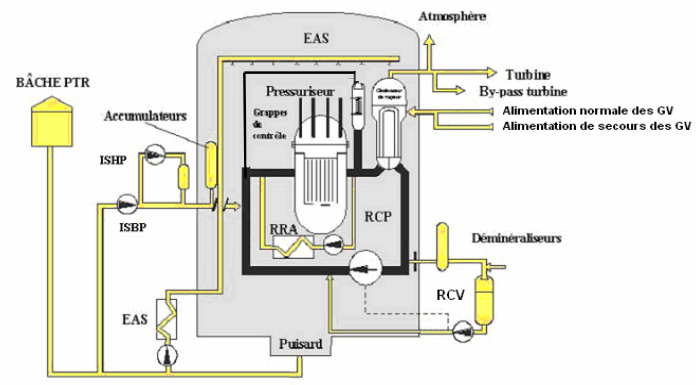
\includegraphics[scale=0.5]{reacteur.png}
\caption{Schéma d'un réacteur nucléaire}
\label{reacteur}
\end{figure}


Un crayon est formé de combustible (uranium et plutonium), mais aussi d'une gaine en Zirconium pour maintenir les pastilles de combustible ensemble. Un accident grave est généralement causé par un problème de refroidissement de ces crayons de combustible dont la puissance résiduelle ne pourra plus être efficacement évacuée. Ces crayons vont alors fondre et former un mélange appelé corium principalement formé de zirconium, d'uranium,de plutonium et parfois de nickel et de chrome venant des installations. La température peut dépasser les 2800K. L'étude de ce mélange est centrale dans l'approche des accidents graves : du fait de sa forte teneur en élément radioactif, ce mélange est destructeur et la propagation de ce mélange peut être fatale à toute l'installation. Le corium se propage alors dans la cuve, puis s'il détruit la cuve, se propage dans le bâtiment du réacteur, et, encore plus grave,à l'éxtérieur du réacteur s'il détruit la structure généralement en béton de celui-ci. Ainsi, en se propageant, le corium réagit avec les différents éléments du réacteur et plusieurs types d'intéraction peuvent alors se produire : intéraction avec l'eau froide du réacteur (ICE), ou encore intéraction avec le béton du fond du réacteur (ICB).  Lorsque le corium commence à se propager dans le réacteur, il y a ainsi de forte chance pour que le réacteur ne puisse plus jamais fonctionner, le but n'est donc pas d'essayer de sauvegarder le réacteur mais de prévenir toute perte humaine. \\

Dans le domaine des accidents graves, les phénomènes physiques mis en jeu sont trés complexes et ne peuvent être bien étudiés à l'heure actuelle. La but de l'étude des accidents graves est de comprendre au mieux ces 
phénomènes, de produire des codes de simulation qui pourront prévoir, toujours au mieux, le comportement du corium mais aussi et sutout d'essayer de majorer l'erreur comise lors de telles simulations. Comme dit précédemment,
les données concernant les accidents graves sont actuellement trés limitées et il est trés difficile de produite de nouvelles données. On peut récupérer des données de prédents accidents (Three Mile Island, Fukushima, Tchernobyl),
ou encore faire des simulations à échelle réduite (installation PLINIUS au Cea Cadarache par exemple). Les codes scénario permettent ainsi de simuler la propagation du corium au sein de l'enceinte du réacteur. Le code PROCOR 
est le code développé au laboratoire LPMA du Cea Cadarache où se déroule le stage. C'est un code orienté objet en Java permettant de créer des applications PROCOR prenant différents modèles (comme un modèle de cuve, un modèle 
de corium) et permettant de simuler les intéractions entre ces modèles. Ainsi une application PROCOR prend la forme d'un système dynamique qui évolue au cours du temps, ce système dynamique étant composé de plusieurs modèles
et d'un ensemble d'intéraction entre ces modèles. Chaque modèle peut évoluer pendant le cycle de vie de l'application, il peut être détruit si par exemple un élément comme le corium détruit une enceinte. La plateforme permet,
 par le biais de méthodes de Monte-Carlo d'obtenir des probabilités de rupture de cuve, ou plus généralement permet d'avoir des résultats de sensibilité sur certain paramètre physique et d'incertitude sur certains matériaux. 
\section{Problématique du stage}
Comme dit précedemment, une application PROCOR est constituée d'un ensemble de composant, ou modèle, interagissant entre eux. Un composant peut être le bain de corium, ou le bain débris que forme le corium en tombant dans 
l'eau du fond de cuve. Chaque modèle est décrit par ses paramètres physiques (chaleur, taille ...), par ses variables (température, masse ...) et enfin par ses équations. Le système d'équation d'un modèle peut 
être un système d'équations différentielles ordinaires, ou encore un système d'équations aux dérivées partielles, ou encore un système linéaire ou une fonction analytique issue de l'expérience. Un modèle a un ou plusieurs états : par 
exemple le bain de corium peut être liquide ou solide. Dans chaque modèle, on a des règles de transition qui permettent de savoir s'il on est dans un état ou un autre. Ces règles prennent généralement la forme de seuil : en fonction
de la valeur d'une certaine fonction par rapport à ce seuil, on est dans un état ou l'autre. 

Une fois les composants définis dans une application PROCOR, il faut définir les intéractions entre ces composants. Ces intéractions prennent généralement la forme de termes d'échanges (échange de masse par exemple entre 
le lit de débris et le bain de corium, ou échange de chaleur du bain de corium vers le lit de débris). D'un point vu du code Java, ces intéractions impliquent que les paramètres en entrée d'un modèle soient liés aux variables de 
sortie d'un autre modèle. La simulation se fait ensuite sur deux pas de temps : un pas de temps interne à chaque composant et un pas de temps externe. A chaque pas de temps externe, on va synchroniser tous les composants entre eux. 
Ce pas de temps externe, qui est fixé de manière heuristique et parfois à l'aide d'expériences physiques, n'est généralement pas optimal et ne permet pas de minimiser l'erreur commise.Ainsi, actuellement, lorsque l'on créé 
une application PROCOR, il faut créer à la main les liaisons entre modèles et définir les différents pas de temps. C'est sur ce point que le stage doit se concentrer : essayer d'automatiser le couplage entre modèle et prévoir
l'erreur commise en fonction de ce couplage.
\newpage
\section{Solutions envisagées}
Pour solutionner ce problème, il faudra tout d'abord étudier le problème sur une application simplifiée (voir figure~\ref{model}) comprenant des liaisons entre modèles poblématiques et mettant bien en valeur l'intêret de ce stage. Ce modèle est
présenté dans le schéma ci dessous. L'application PROCOR a créer devra simuler l'intéraction entre un lit de débris et un bain de corium. Le lit de débris, comme le bai nde corium, aura deux états : un état à une couche
et un état à deux couches. On peut avoir des échanges internes entre chaque couche du composant, et l'on a aussi des échanges entre les composants du modèle. Ces intéractions ont été créé pour être problématiques et pour mettre
en valeur l'importance qu'à le couplage entre les composants d'une application PROCOR. 
\begin{figure}[h]
\centering
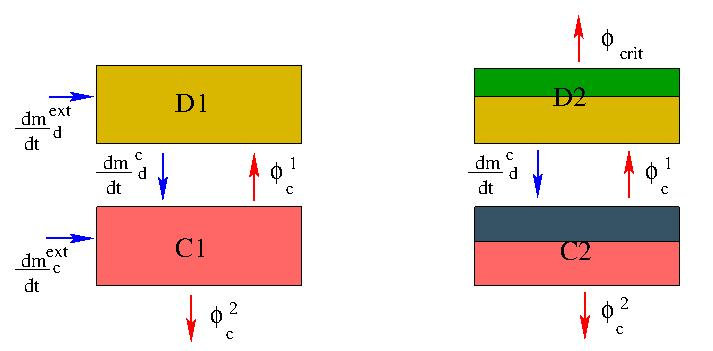
\includegraphics[scale=0.5]{model.jpeg}
\caption{Modèle simplifé : en haut le lit de débris, en bas le bain de corium. De gauche à droite, les deux états de chaque composant}
\label{model}
\end{figure}

Ensuite, une fois le problème bien compris sur le modèle simplifié, on pourra utiliser un schéma de prédicteur/correcteur pour améliorer le couplage sur la boucle temporelle externe des différents composants d'une application
PROCOR. Ce schéma permettra de simuler le déroulement de l'application et ainsi d'optimiser l'application en estimant l'erreur commise en fonction du couplage effectué. On pourra aussi, pour automatiser le couplage, essayer
de construire une architecture de code en programmation objet en Java permettant cette automatisation pour faciliter la construction d'application PROCOR.\\ 

Si ceci est terminé avant la fin du stage, il serait aussi interessant d'étudier le comportement interne des composants du modèle et essayer de synchroniser leur paramètre avec d'autres composants par le biais de 
"Message Passing". Ainsi si par exemple, le lit de débris se liquifie à un instant à l'intérieur de la boucle temporelle, un message sera envoyé aux autres composants pour prévenir d'un changement d'état. On pourra 
ainsi améliorer la robustesse et la précision de la simulation. Le résultat vraiment attendu du stage est l'implantation du schéma prédicteur/correcteur, le codage du "Message Passing" ne sera fait que si il reste du temps
à la fin du stage.  
\end{document}